

\tikzset{every picture/.style={line width=0.75pt}} %set default line width to 0.75pt

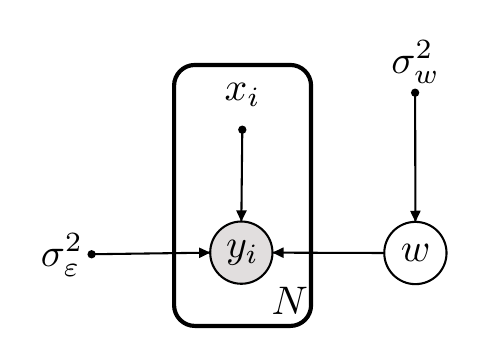
\begin{tikzpicture}[x=0.75pt,y=0.75pt,yscale=-0.6,xscale=0.6]
%uncomment if require: \path (0,300); %set diagram left start at 0, and has height of 300

\draw    (455.78, 219.29) circle [x radius= 25, y radius= 25]  ;
\draw  [fill={rgb, 255:red, 225; green, 222; blue, 222 }  ,fill opacity=1 ]  (316, 219) circle [x radius= 25, y radius= 25]  ;
\draw    (430.78,219.29) -- (341,219) ;
\draw [shift={(341,219)}, rotate = 360.18] [fill={rgb, 255:red, 0; green, 0; blue, 0 }  ] [draw opacity=0] (8.93,-4.29) -- (0,0) -- (8.93,4.29) -- (8.93,-4.29)    ;

\draw  [line width=1.5]  [rounded corners= 7.5] (262, 68.29) rectangle (372, 277.86)   ;
\draw    (195.78,220.29) -- (291,219) ;
\draw [shift={(291,219)}, rotate = 539.23] [fill={rgb, 255:red, 0; green, 0; blue, 0 }  ] [draw opacity=0] (8.93,-4.29) -- (0,0) -- (8.93,4.29) -- (8.93,-4.29)    ;
\draw [shift={(195.78,220.29)}, rotate = 359.23] [fill={rgb, 255:red, 0; green, 0; blue, 0 }  ] [draw opacity=0]    (0, 0) circle [x radius= 3.35, y radius= 3.35]   ;
\draw    (455.56,90.57) -- (455.78,194.29) ;
\draw [shift={(455.78,194.29)}, rotate = 269.88] [fill={rgb, 255:red, 0; green, 0; blue, 0 }  ] [draw opacity=0] (8.93,-4.29) -- (0,0) -- (8.93,4.29) -- (8.93,-4.29)    ;
\draw [shift={(455.56,90.57)}, rotate = 89.88] [fill={rgb, 255:red, 0; green, 0; blue, 0 }  ] [draw opacity=0]    (0, 0) circle [x radius= 3.35, y radius= 3.35]   ;
\draw    (316.78,120.29) -- (316,194) ;
\draw [shift={(316,194)}, rotate = 270.61] [fill={rgb, 255:red, 0; green, 0; blue, 0 }  ] [draw opacity=0] (8.93,-4.29) -- (0,0) -- (8.93,4.29) -- (8.93,-4.29)    ;
\draw [shift={(316.78,120.29)}, rotate = 90.61] [fill={rgb, 255:red, 0; green, 0; blue, 0 }  ] [draw opacity=0]    (0, 0) circle [x radius= 3.35, y radius= 3.35]   ;

\draw (456,219) node [scale=1.44]  {$\boldsymbol{w}$};
\draw (317,219) node [scale=1.44]  {$y_{i}$};
\draw (355,258) node [scale=1.44]  {$N$};
\draw (172,221) node [scale=1.44]  {$\sigma ^{2}_{\varepsilon }$};
\draw (456,66) node [scale=1.44]  {$\sigma ^{2}_{w}$};
\draw (317,92) node [scale=1.44]  {$x_{i}$};


\end{tikzpicture}
